%% Implementation Phase Presentation Template (KIT Beamer)
\documentclass{sdqbeamer}[en]
\usepackage{booktabs}
\usepackage{amssymb}
\usepackage{adjustbox}

\grouplogo{codex_logo} 
\groupname{ITEC - Institute of Computer Engineering}

\title[Quality Assurance]{CodeX: Natural Language to Structured Code Generation}
\subtitle{Quality Assurance} 
\author[Pavlov Kyrylo]{Oleksandr Brittner, Simon Bumiller, Simon Gaber, Dayana Karadzhova, \textbf{Kyrylo Pavlov} \newline}
\date[20.\,03.\,2026]{March 20, 2026}

\usepackage{lipsum}
\usepackage{pdfpages}
\usepackage{listings}
\usepackage{pifont}

\newcommand{\cmark}{\ding{51}} % checkmark
\newcommand{\xmark}{\ding{55}} % cross
\newcommand{\omark}{\ding{108}} % circle

\begin{document}

% Titelseite
\begin{frame}[title green horizontal, picture=images/qa_3, kitlogo=white] \titlepage 
\end{frame}
% Inhaltsverzeichnis
\begin{frame}[tableofcontents=green]{Content}
\tableofcontents
\end{frame}

\section{Tests}

\begin{frame}{Unit Tests}{Background}
  \textbf{What are Unit Tests?}\\[0.5em]
  Unit tests verify individual components of the system in isolation,
  ensuring each function or module behaves correctly before integration.\\[1em]

  \textbf{Technologies Used}
  \begin{columns}
    \column{0.5\textwidth}
    \textbf{Client -- Vitest}
    \begin{itemize}
      \item TypeScript-native test framework
      \item Tests \texttt{.ts} files
      \item Covers ViewModels, Service\\Implementations, Local Data Caching
      \item Mocks for browser APIs \&\\external services
    \end{itemize}
    \column{0.5\textwidth}
    \textbf{Server -- pytest}
    \begin{itemize}
      \item Python testing framework
      \item Tests \texttt{.py} files
      \item Covers Service Endpoints,\\Managers \& Persistence Repositories
      \item Central bootstrap via\\
            \texttt{tests/conftest.py}\\
            (no external services needed)
    \end{itemize}
  \end{columns}
\end{frame}

\begin{frame}{Unit Tests}
  \begin{columns}
    \column{0.5\textwidth}
    \textbf{Client (Vitest)}
    \begin{itemize}
      \item 176 tests
      \item Statement coverage: 76.79\%
      \item Branch coverage: 86.9\%
      \item Function coverage: 84.83\%
    \end{itemize}
    \column{0.5\textwidth}
    \textbf{Server (pytest)}
    \begin{itemize}
      \item 227 tests
      \item Statement coverage: 94\%
      \item Branch coverage: 83\%
    \end{itemize}
  \end{columns}
\end{frame}

\begin{frame}{End-to-End Tests}{Test Cases}
  \begin{columns}[T]
    \column{0.5\textwidth}
    \begin{itemize}
      \item \textbf{T10} Authentication via OAuth provider
      \item \textbf{T20} Authentication via credentials
      \item \textbf{T30} Updating user data
      \item \textbf{T40} Making a request
    \end{itemize}
    \column{0.5\textwidth}
    \begin{itemize}
      \item \textbf{T50} Manipulating language models
      \item \textbf{T60} Manipulating conversations
      \item \textbf{T70} Admin actions
      \item \textbf{T80} Change theme and language
    \end{itemize}
  \end{columns}
\end{frame}

\begin{frame}{End-to-End Tests}
  \textbf{Tool:} Playwright (automated browser simulation)
  \vspace{0.5em}
  \begin{itemize}
    \item \textbf{T20, T40--T80:} Implemented
    \item \textbf{T30:} Partially implemented (email verification not automatable)
    \item \textbf{T10:} Not implemented (Google OAuth blocked by captcha)
  \end{itemize}
\end{frame}

\begin{frame}{Server Load Tests}{Device Specs}
  \vspace{-0.5em}
  \textbf{Tests were executed on the following machine:}\\[0.8em]

  \begin{itemize}
    \item \textbf{CPU:} Intel Pentium G4400T @ 2.90 GHz (2 cores)
    \item \textbf{Memory:} 15 GB RAM
    \item \textbf{Storage:} 476.9 GB NVMe SSD
    \item \textbf{OS:} Debian GNU/Linux 13 (Trixie)
    \item \textbf{Kernel:} 6.12.63+deb13-amd64
  \end{itemize}

  \vfill
  
  {\small Load tests were executed from a separate machine located in a different network.}
\end{frame}

\begin{frame}{Server Load Tests}
  \textbf{Ramp-up model:} 1 → 2 → 3 users/sec, 3 sec each\\[0.5em]
  Scenarios tested: Settings, LLM Config, Authentication, Conversations\\[0.5em]
  \begin{itemize}
    \item Response times correlate with SQL/vector/LLM access
    \item Settings \& LLM config: low latency
    \item Authentication: medium latency
    \item Conversations: high latency, some timeouts under load
  \end{itemize}
\end{frame}

\begin{frame}{Server Load Tests}{Settings \& LLM}
  \begin{figure}
    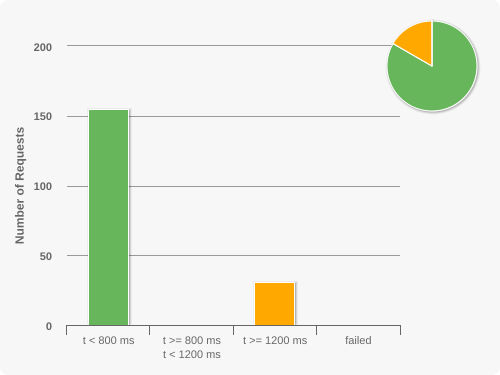
\includegraphics[width=0.45\textwidth]{images/set.png}
    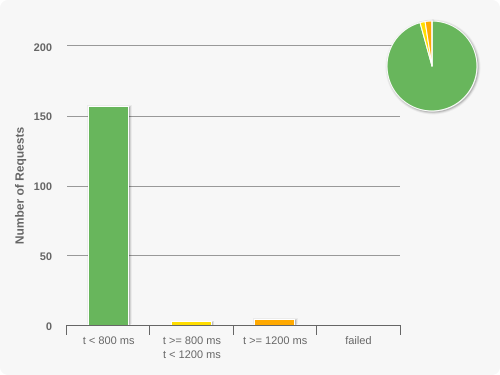
\includegraphics[width=0.45\textwidth]{images/llm.png}
  \end{figure}
\end{frame}

\begin{frame}{Server Load Tests}{Authentication \& Conversation}
  \begin{figure}
    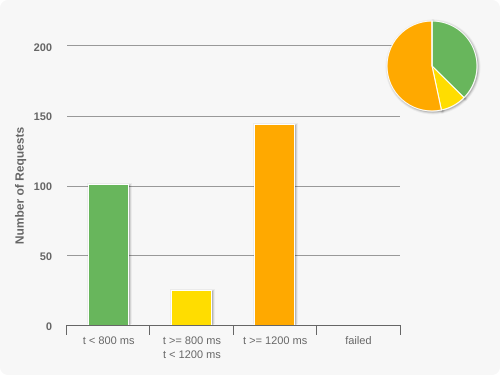
\includegraphics[width=0.45\textwidth]{images/auth.png}
    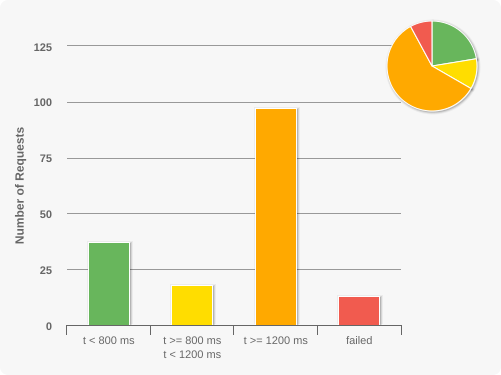
\includegraphics[width=0.45\textwidth]{images/conv.png}
  \end{figure}
\end{frame}

%% ------------------------
\section{Software Quality}

\begin{frame}{Software Quality}
  \begin{itemize}
    \item \textbf{Static Analysis:} TypeScript + ESLint (client), linting tools (server)
    \item \textbf{Extensibility:} Layered ViewModel architecture; modular server
    \item \textbf{Testability:} Business logic cleanly separated from UI; mocks for external deps
    \item \textbf{Readability:} Consistent naming, centralized configs, added comments
  \end{itemize}
\end{frame}


%% ------------------------
\section{Bugs}

\begin{frame}{Bugs}{Addressed Issues}
  \begin{columns}
    \column{0.33\textwidth}
    \textbf{UI}
    \begin{itemize}
      \item Unrecognizable buttons
      \item Dark mode colors
      \item Font size too small
    \end{itemize}
    \column{0.33\textwidth}
    \onslide<2->{
    \textbf{Client}
    \begin{itemize}
      \item Send button broken on some browsers
      \item Wrong post-logout URL
      \item Token saving bug
    \end{itemize}
    }
    \column{0.33\textwidth}
    \onslide<3->{
    \textbf{Server}
    \begin{itemize}
      \item JWT timezone bug
      \item ChromaDB trash chunks
      \item OAuth email confirmation
      \item Model deletion crash
    \end{itemize}
    }
  \end{columns}
\end{frame}




%% ------------------------
\section{User Test}

\begin{frame}{User Tests}
  \begin{itemize}
    \item Total 4 participants
    \item All participants completed tasks successfully
    \item Navigation perceived as intuitive
    \item Ratings: predominantly \textit{good} to \textit{very good}
    \item Positives: clear structure, fast response time
    \item Improvements needed: clarity of some dialogs \& interactive elements
  \end{itemize}
\end{frame}

\begin{frame}{User Tests}{Feedback}
  \begin{columns}
    \column{0.5\textwidth}
    \begin{itemize}
      \item Incorrect error message for username requirements
      \item No element specialization during visualization
      \item Connections not visible in dark mode
      \item Prompt text too small / unnoticeable
    \end{itemize}
    \column{0.5\textwidth}
    \begin{itemize}
      \item After deleting a chat, no other chat opens
      \item Chat search is case-sensitive
      \item Misaligned registration window
      \item Sliders at the bottom lack clear purpose
    \end{itemize}
  \end{columns}
\end{frame}

\begin{frame}{User Tests}{Feedback}
  \begin{columns}
    \column{0.5\textwidth}
    \begin{itemize}
      \item Incorrect error message for username requirements \textcolor{green}{\checkmark}
      \item No element specialization during visualization \textcolor{green}{\checkmark}
      \item Connections not visible in dark mode \textcolor{green}{\checkmark}
      \item Prompt text too small / unnoticeable \textcolor{green}{\checkmark}
    \end{itemize}
    \column{0.5\textwidth}
    \begin{itemize}
      \item After deleting a chat, no other chat opens \textcolor{green}{\checkmark}
      \item Chat search is case-sensitive \textcolor{orange}{$\circ$}
      \item Misaligned registration window \textcolor{green}{\checkmark}
      \item Sliders at the bottom lack clear purpose \textcolor{orange}{$\circ$}
    \end{itemize}
  \end{columns}
  \vspace{1em}
  {\small \textcolor{green}{\checkmark} Fixed \quad \textcolor{orange}{$\circ$} Optional / Not yet fixed}
\end{frame}
%% ------------------------
\section{New Functions}

\begin{frame}{New Functions}{Embedding Function}
  \vspace{-0.5em}
  \begin{columns}[T]
    \column{0.55\textwidth}
    \textbf{Two embedding functions now available:}\\[0.6em]

    \textbf{Default ChromaDB Embedding}
    \begin{itemize}
      \item No API key required
      \item Runs fully locally
      \item Free
    \end{itemize}
    \vspace{0.4em}
    \textbf{OpenAI Embedding Function}
    \begin{itemize}
      \item Higher semantic accuracy
      \item Better for complex queries
      \item Not free
    \end{itemize}

    \column{0.45\textwidth}
    \vspace{-0.5em}
    \begin{figure}
      \centering
      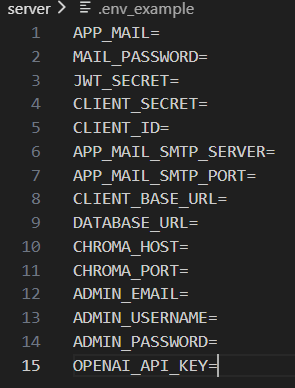
\includegraphics[width=0.5\textwidth]{images/env_empl.png}
    \end{figure}
  \end{columns}
  \vfill
  
  {\small Users can switch between embedding functions in the .env file}
\end{frame}

\begin{frame}{New Functions}{Universal LLM Support}
  \vspace{-0.5em}
  \begin{columns}[T]
    \column{0.55\textwidth}
    \textbf{All LLM models are now supported}\\[0.8em]

    Previously limited to OpenAI-type models only.\\[0.6em]

    \textbf{How?} -- via \textbf{LiteLLM}
    \begin{itemize}
      \item Unified interface for 100+ LLM providers
      \item Models from OpenAI, Anthropic, Mistral, Ollama and more
      \item No provider-specific integration needed
    \end{itemize}
    \vspace{0.6em}
    \textbf{Before:} Only OpenAI-type models\\
    \textbf{After:} Any model via LiteLLM

    \column{0.45\textwidth}
    \vspace{-0.5em}
    \begin{figure}
      \centering
      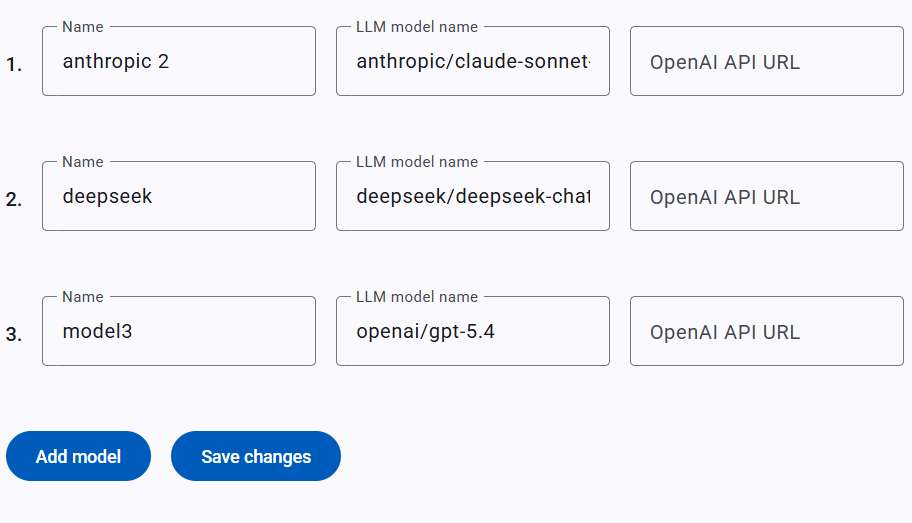
\includegraphics[width=\textwidth]{images/llmset.png}
    \end{figure}
  \end{columns}
\end{frame}

\begin{frame}{New Functions}{Simulation Visualization}
\vspace{-0.2em}

\begin{columns}[T]

    % TEXT COLUMN (smaller)
    \column{0.42\textwidth}
    \textbf{Simulation Visualization}\\[0.5em]
    Users can now view not only:
    \begin{itemize}
      \item SPICE netlist code
      \item Circuit graph representation
    \end{itemize}

    \vspace{0.4em}
    \textbf{But also:} an interactive simulation graph\\[0.6em]

    \textbf{How it works:}
    \begin{itemize}
      \item Parses \texttt{.PRINT} statements from the netlist
      \item Visualizes only printable variables
      \item e.g. \texttt{.PRINT TRAN V(6) V(2) V(1)}
    \end{itemize}

    % IMAGE COLUMN (larger + centered feel)
    \column{0.58\textwidth}
    \begin{figure}
      \centering
      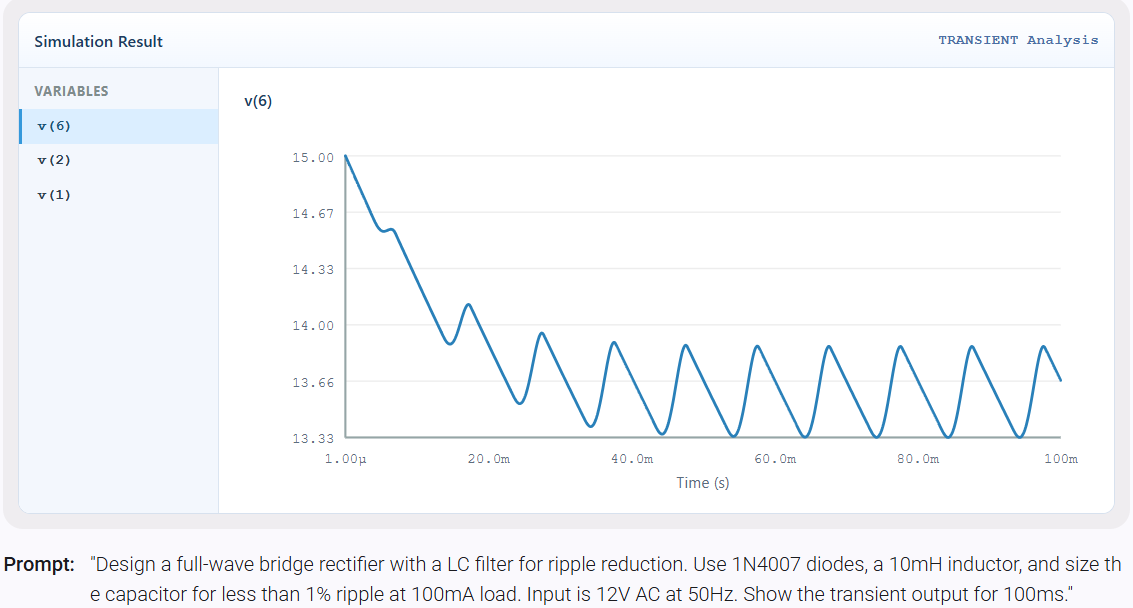
\includegraphics[width=0.95\textwidth]{images/simul.png}
    \end{figure}

\end{columns}
\end{frame}


\begin{frame}[c]{Conclusion}

\begin{center}

\onslide<1->{\Large Thank you for your attention!}

\end{center}

\end{frame}


%% ------------------------



%% ------------------------

\end{document}
